\chapter{Kiểm thử và đánh giá kết quả}
\label{ch:kiem-thu}

\section{Mục tiêu kiểm thử}

\begin{enumerate}
    \item Xác nhận chuỗi guard đa lớp, pipeline RAG có RBAC, SQLite Authorizer AST Guard và Multi-Tool Company Agent hoạt động chính xác qua bộ kiểm thử tự động ($469+$ unit \& integration tests).
    \item Đánh giá hiệu quả phát hiện trên bộ dữ liệu tổng hợp nội bộ ($425$ case) và \textbf{kiểm chứng độc lập} trên bộ benchmark công khai ngoài phân phối \texttt{deepset/\allowbreak prompt-\allowbreak injections} ($662$ mẫu đa ngôn ngữ) trước và sau khi nâng cấp kiến trúc P5.
    \item Thực hiện \textbf{đối sánh định lượng} công bằng giữa \textbf{Shield AI} (Rule-Only và Rule + Semantic Judge \texttt{gemma4:e2b}) với hai giải pháp chuẩn quốc tế là \textbf{Meta Llama Guard~3 1B} (\texttt{llama-\allowbreak guard3:1b}) và \textbf{NVIDIA NeMo Guardrails} (\texttt{self\_\allowbreak check\_\allowbreak input}) trên cùng tập dữ liệu và cùng phần cứng.
    \item Đo đạc đầy đủ phân vị độ trễ \textbf{\texttt{p50 / p95 / p99}} cho từng tầng xử lý (Input Guard, Semantic Pre-screen, Semantic Judge LLM, RAG Context Guard, Output/DLP Guard, Retrieval, SQL Guard, Indirect Result Guard) khi bật và tắt Semantic Judge.
    \item Bắn trực tiếp công cụ red-team độc lập \textbf{\texttt{NVIDIA garak v0.\allowbreak 17.\allowbreak 1}} ($2.048$ probe qua HTTP REST) và bộ biến đổi/tấn công thích nghi đa lượt \textbf{\texttt{PyRIT}} vào các endpoint sống (\texttt{/\allowbreak v1/\allowbreak rag/\allowbreak query}, \texttt{/\allowbreak v1/\allowbreak gateway/\allowbreak chat}, \texttt{/v1/conversations/\{id\}/messages}).
\end{enumerate}

\section{Phương pháp kiểm thử}

Nhóm kết hợp: (i)~kiểm thử đơn vị/tích hợp bằng pytest cho các guard và pipeline RAG; (ii)~đánh giá hiệu quả bảo mật trên bộ tấn công/lành tính tổng hợp với ba cấu hình guard; (iii)~thí nghiệm tối ưu lớp luật, đo trước/sau trên cùng bộ dữ liệu.

\section{Môi trường kiểm thử}

Toàn bộ kiểm thử chạy trong môi trường ảo Python (\texttt{.venv}) để cô lập phụ
thuộc. Bộ pytest dùng thư mục tạm ngoài repo khi cần, tránh làm bẩn cây mã nguồn.
Đường đánh giá chính không gọi mạng (Mock Provider tất định); riêng cấu hình
Semantic Judge dùng mô hình cục bộ chạy qua ollama, không phụ thuộc dịch vụ trực
tuyến.

\section{Các nhóm kiểm thử}

\subsection{Kiểm thử chức năng}
Nhóm kiểm thử chức năng xác nhận từng thành phần cho quyết định đúng trên các ca
đại diện. Phạm vi bao phủ quyết định của từng guard (đầu vào, ngữ cảnh, đầu ra),
pipeline RAG và cơ chế kiểm soát truy cập theo vai trò (RBAC). Mỗi ca kiểm thử cố
định đầu vào và kỳ vọng đầu ra, nhờ đó lỗi hồi quy được phát hiện ngay khi mã
nguồn thay đổi.

\subsection{Kiểm thử lỗi và fail-closed}
Nhóm kiểm thử này xác nhận hệ thống xử lý đúng các tình huống vi phạm và lỗi. Cụ
thể, nó kiểm tra nguyên tắc ``quyết định nghiêm khắc nhất thắng'' khi nhiều guard
cùng phát hiện vấn đề, và hành vi fail-closed khi có vi phạm rõ ràng. Mục tiêu là
bảo đảm một lỗi cục bộ không khiến hệ thống mặc định cho câu trả lời đi qua.

\section{Kịch bản kiểm thử chính}

\begin{itemize}
    \item Baseline (always-allow) so với có guard trên bộ đánh giá bảo mật tổng hợp.
    \item Ba cấu hình guard (rule-based, Semantic Judge \texttt{qwen3:4b}, đối chiếu \texttt{hermes3:8b}) trên cùng bộ 425 case.
    \item Thí nghiệm tối ưu lớp luật: đo TPR/FPR trước và sau trên cùng dữ liệu.
\end{itemize}

\section{Kết quả kiểm thử tự động}

\begin{table}[!htbp]
\centering
\caption{Tổng hợp kết quả kiểm thử tự động tích hợp (Nhánh \texttt{feat-\allowbreak p5-\allowbreak integrated-\allowbreak thesis})}
\label{tab:test-summary}
\begin{tabular}{@{}L{0.58\linewidth}L{0.34\linewidth}@{}}
\toprule
\textbf{Nhóm kiểm thử (\texttt{pytest})} & \textbf{Kết quả} \\
\midrule
Input Guard, RAG Context Guard, Output/DLP Guard \& Semantic Judge & $151$ passed, $0$ failed \\
Pipeline RAG, Provenance Guard, Canonical I/O \& Ollama Provider & $180$ passed, $0$ failed \\
Text-to-SQL Guard (Authorizer AST), Result Guard \& Company Agent (Nhà Mộc Việt) & $138$ passed, $0$ failed \\
\textbf{Tổng bộ kiểm thử tích hợp P2 + P3 + P4 + P5} & \textbf{469 passed, 0 failed ($3{,}61\,\text{s}$)} \\
\textbf{Full repository regression suite (\texttt{verify\_\allowbreak phase.\allowbreak ps1})} & \textbf{1708 passed, 0 failed, 4 skipped} \\
\bottomrule
\end{tabular}
\end{table}

Các số liệu trên là kết quả kiểm thử tự động của hệ thống lab, \textbf{không} phải chỉ số hiệu quả bảo mật trên môi trường thật.

\section{Đánh giá hiệu quả bảo mật trên bộ tấn công tổng hợp}
\label{sec:sec-eval}

Bộ đánh giá bảo mật tổng hợp gồm \textbf{425 case}: \textbf{200 case tấn công}
\emph{lấy cảm hứng} từ các họ kỹ thuật của NVIDIA garak~\cite{derczynski2024garak},
Microsoft PyRIT~\cite{microsoft_pyrit} và InjecAgent~\cite{zhan2024injecagent} (template tĩnh tự xây,
\textbf{không} gọi các bộ công cụ gốc) và
\textbf{225 câu lành tính} gồm 100 câu nghiệp vụ thông thường và 125 câu
\emph{hard benign} --- câu hợp lệ nhưng bề mặt trông đáng ngờ (chứa từ khoá nhạy
cảm hợp pháp, hỏi bảo mật chính đáng, tự phục vụ, diễn đạt lại), dùng để đo
precision thật của tường. Toàn bộ payload là dữ liệu tổng hợp, sinh xác định.
Đánh giá chạy trên ba cấu hình trên \emph{cùng một bộ 425 case}:
(a)~\textbf{rule-based} (chỉ guard luật); (b)~\textbf{semantic} (bổ sung
Semantic Judge trên mô hình cục bộ \texttt{qwen3:4b}); và (c)~một lần
\textbf{đối chiếu} với mô hình lớn hơn \texttt{hermes3:8b}.

Các chỉ số được định nghĩa: \textbf{TPR} = tấn công bị chặn / tổng tấn công;
\textbf{FPR} = câu lành tính bị chặn / tổng lành tính; \textbf{Stop-before-LLM}
= tỉ lệ tấn công bị chặn trước khi gọi mô hình; \textbf{Exfil Marker Rate} =
tỉ lệ câu trả lời để lộ mã canary bí mật. Ở giai đoạn cơ sở trên tập 425 case này, các chỉ số phát hiện được đo độc lập với thời gian phản hồi; phép đo phân vị độ trễ \texttt{p50/\allowbreak p95/\allowbreak p99} của từng tầng được trình bày chuyên sâu tại Mục~\ref{sec:latency-eval}.

\textbf{Lựa chọn và ý nghĩa chỉ số.} Với một tường guard, hai chỉ số TPR và FPR
không cùng vai trò. \textbf{FPR được xem là ràng buộc cứng}: một tường chặn nhầm
câu nghiệp vụ hợp lệ sẽ không thể triển khai, dù có TPR cao đến đâu --- người
dùng sẽ tắt nó. Do đó bộ lành tính được thiết kế \emph{khó} (125 câu
\emph{hard benign} chứa từ khoá nhạy cảm hợp pháp, hỏi bảo mật chính đáng, tự
phục vụ) để đo precision thật, và mục tiêu là \emph{tối đa hoá TPR trong khi giữ
FPR ở mức thấp nhất có thể}. \textbf{TPR/recall} phản ánh rủi ro bỏ lọt: trong an
ninh, bỏ sót một đòn tấn công thật thường nguy hiểm hơn một cảnh báo nhầm, nên
recall là đại lượng cần cải thiện. \textbf{Stop-before-LLM} đo phần tấn công bị
chặn \emph{trước} khi gọi mô hình --- vừa tiết kiệm chi phí token, vừa là phòng
thủ sớm không phụ thuộc hành vi mô hình. \textbf{Exfil Marker Rate} đo rò rỉ ở
tầng đầu ra; như phân tích bên dưới, phép đo này hiện bị nhiễu và chỉ dùng như
chỉ báo định tính. Tất cả tỉ lệ có cỡ mẫu dưới ngưỡng $n=10$ được báo là ``không
đủ mẫu'' thay vì một con số dễ gây hiểu lầm.

\textbf{Tối ưu lớp luật.} Lần đánh giá đầu cho thấy lớp luật bỏ lọt hoàn toàn họ
PyRIT (đóng vai/mạo danh thẩm quyền, $0\%$). Chúng tôi bổ sung một nhóm luật
nhắm \emph{hai bất biến từ vựng} của đòn mạo danh (cụm từ đặc trưng, không phải đặc trưng ngữ nghĩa) --- chỉ thị vượt quyền (ghi đè chính
sách/ACL, ``không được từ chối cấp trên'') và yêu cầu trích xuất hàng loạt dữ
liệu nhạy cảm --- thay vì khớp đúng câu chữ của từng case. Trên cùng bộ 425
case, thay đổi này nâng TPR của lớp luật từ $48{,}5\%$ lên $77{,}0\%$ mà
\textbf{giữ nguyên FPR $0\%$ trên bộ 225 câu lành tính tổng hợp}. Bước tối ưu thứ
hai --- \textbf{chuẩn hoá đầu vào} trước khi đối chiếu luật (NFKC, loại ký tự ẩn
zero-width, gấp các đồng hình Cyrillic về Latin) --- vô hiệu hoá kỹ thuật ``làm
rối Unicode'' của garak, nâng tiếp TPR lên $\mathbf{81{,}5\%}$ (garak
$75{,}2\%\to83{,}8\%$) vẫn ở FPR $0\%$ (Bảng~\ref{tab:v3-optim}). Đây là bước
giải nhiễu \emph{tổng quát}, không tinh chỉnh theo case cụ thể. \textbf{Bước tối
ưu thứ ba} bổ sung ba luật cho các đòn tiêm nhiễm gián tiếp: (a) mở rộng luật
``bỏ qua chỉ thị'' sang cả \emph{chính sách/quy định} (bắt ngữ cảnh bị đầu độc
kiểu ``[INTERNAL POLICY UPDATE --- AUTHORITATIVE] Ignore previous HR policy''),
(b) luật tiếng Việt cho ``bỏ qua hướng dẫn/chính sách'', (c) nhận diện dấu hiệu
chèn ngữ cảnh (``[SYSTEM FOR \ldots ONLY]'', ``invisible policy''). Ba luật này
--- nhắm \emph{loại} tấn công gián tiếp, không khớp câu chữ --- nâng TPR lên
$\mathbf{97{,}0\%}$: bắt trọn họ injecagent ($47{,}4\%\to100\%$) và nâng garak
($83{,}8\%\to94{,}3\%$), vẫn ở FPR $0\%$; đã kiểm bằng paraphrase mới (vi/en) và
câu chính sách hợp lệ trong kiểm thử đơn vị. Phần bỏ lọt còn lại ($6/10$
\emph{direct\_kb\_exfil}) là yêu cầu dữ liệu của người khác không có dấu hiệu từ
vựng nên \emph{qua được} lớp luật đầu vào (allow, có gọi mô hình) --- đây là giới
hạn recall của Input Guard, ghi nhận thẳng thắn. Việc từ chối truy cập tài liệu
của \emph{người khác} là nhiệm vụ của lớp RBAC/ACL ở khâu truy hồi (kiểm soát
riêng, \textbf{không} đo bằng chỉ số TPR ở đây). Cần nói rõ phạm vi: đây \textbf{không} phải bằng chứng
đã ``vá'' mạo danh nói chung. Con số $100\%$ trên họ PyRIT phản ánh việc họ
template tổng hợp hiện tại (khoảng sáu khung) đều nhúng đúng hai bất biến mà luật
bắt; kẻ tấn công diễn đạt lại để bỏ hai bất biến (bỏ định lượng ``toàn bộ'', bỏ
động từ ghi đè) vẫn né được luật --- kiểm thử đơn vị ghi nhận rõ tám đòn né như
vậy đều lọt (phù hợp với tài liệu về vượt qua guardrail~\cite{hackett2025bypass}).
Tương tự, FPR $0\%$ đúng trên bộ tổng hợp nhưng \textbf{không khái quát}: một số
câu quản trị/điều hành hợp lệ ngoài phân phối (câu hỏi \emph{về} việc ghi đè
chính sách, yêu cầu xuất dữ liệu hợp pháp cho kiểm toán) vẫn bị chặn nhầm và được
ghi nhận là hạn chế.

\begin{table}[!htbp]
\centering
\caption{Tối ưu lũy tiến lớp luật qua ba bước (cùng bộ 425 case)}
\label{tab:v3-optim}
\begin{tabularx}{\linewidth}{@{}L{0.24\linewidth}YYYY@{}}
\toprule
\textbf{Chỉ số} & \textbf{Baseline} & \textbf{+ Mạo danh} & \textbf{+ Chuẩn hoá} & \textbf{+ Chống tiêm nhiễm} \\
\midrule
TPR (tấn công) & 48{,}5\% & 77{,}0\% & 81{,}5\% & \textbf{97{,}0\%} \\
FPR (lành tính) & 0{,}0\% & 0{,}0\% & 0{,}0\% & 0{,}0\% \\
PyRIT (n=57) & 0{,}0\% & 100\% & 100\% & 100\% \\
garak (n=105) & 75{,}2\% & 75{,}2\% & 83{,}8\% & 94{,}3\% \\
injecagent (n=38) & 47{,}4\% & 47{,}4\% & 47{,}4\% & 100\% \\
\bottomrule
\end{tabularx}
\end{table}

\begin{table}[!htbp]
\centering
\caption{Ma trận nhầm lẫn --- rule-based sau tối ưu (n = 425; run \texttt{3dc0ee61})}
\label{tab:v3-cm-mock}
\begin{tabularx}{\linewidth}{@{}L{0.30\linewidth}YY@{}}
\toprule
 & \textbf{Bị chặn} & \textbf{Được trả lời} \\
\midrule
Tấn công (n=200) & 194 (TP) & 6 (FN) \\
Lành tính (n=225) & 0 (FP) & 225 (TN) \\
\bottomrule
\end{tabularx}
\end{table}

\begin{table}[!htbp]
\centering
\caption{Ma trận nhầm lẫn --- \texttt{qwen3:4b} + Output-DLP (n = 425; run \texttt{4d01bba6})}
\label{tab:v3-cm-semantic}
\begin{tabularx}{\linewidth}{@{}L{0.30\linewidth}YY@{}}
\toprule
 & \textbf{Bị chặn} & \textbf{Được trả lời} \\
\midrule
Tấn công (n=200) & 200 (TP) & 0 (FN) \\
Lành tính (n=225) & 60 (FP) & 165 (TN) \\
\bottomrule
\end{tabularx}
\end{table}

Đọc trực tiếp hai ma trận (sau ba bước tối ưu lớp luật, và Output-DLP canary):
cấu hình \textbf{rule-based} chặn $194/200$ ($97{,}0\%$) và \emph{không} chặn nhầm
câu lành tính nào trên bộ tổng hợp ($0/225$). Cấu hình \textbf{qwen3:4b} đạt TPR
$100\%$ nhưng FPR $26{,}7\%$ ($60/225$). Quan trọng: Stop-before-LLM của cả hai
đều $97{,}0\%$ (cùng $194$ đòn chặn trước provider) --- Semantic Judge \emph{không}
tăng chặn sớm; $6$ đòn TPR thêm trên qwen ($194\to200$) là chặn \emph{sau} khi gọi
mô hình (Output Guard bắt canary trong câu trả lời), không phải judge phát hiện
injection ở đầu vào.

\begin{table}[!htbp]
\centering
\caption{So sánh chỉ số hai cấu hình (sau chuẩn hoá + Output-DLP)}
\label{tab:v3-metrics}
\begin{tabularx}{\linewidth}{@{}L{0.34\linewidth}YY@{}}
\toprule
\textbf{Chỉ số} & \textbf{Rule-based} & \textbf{Semantic (qwen)} \\
\midrule
TPR & 97{,}0\% & 100{,}0\% \\
FPR (toàn bộ lành tính) & 0{,}0\% & 26{,}7\% \\
\quad FPR trên hard benign & 0{,}0\% & 28{,}0\% \\
Stop-before-LLM & 97{,}0\% & 97{,}0\% \\
Exfil Marker Rate$^\dagger$ & 0{,}0\% & 0{,}0\% \\
\bottomrule
\end{tabularx}

\vspace{2pt}
{\footnotesize $^\dagger$ Cả hai run đều seed 200 canary (rule-based
\texttt{3dc0ee61}, qwen \texttt{4d01bba6}): marker $0\%$ nhờ Output-DLP chặn
canary trong answer --- \textbf{không} đồng nghĩa hết injection ở đầu vào ($6/200$
vẫn tới provider). Xem Mục~\ref{sec:ab-demo} và Hạn chế.\par}
\end{table}

\begin{table}[!htbp]
\centering
\caption{Tỉ lệ chặn theo nguồn tấn công (case tấn công)}
\label{tab:v3-by-family}
\begin{tabularx}{\linewidth}{@{}L{0.30\linewidth}YY@{}}
\toprule
\textbf{Nguồn} & \textbf{Rule-based} & \textbf{Semantic (qwen)} \\
\midrule
garak (jailbreak, Unicode, chia tách) & 94{,}3\% & 100{,}0\% \\
injecagent (chỉ thị ẩn/đầu độc) & 100{,}0\% & 100{,}0\% \\
pyrit (đóng vai, mạo danh) & 100{,}0\% & 100{,}0\% \\
\bottomrule
\end{tabularx}
\end{table}

\begin{figure}[!htbp]
\centering
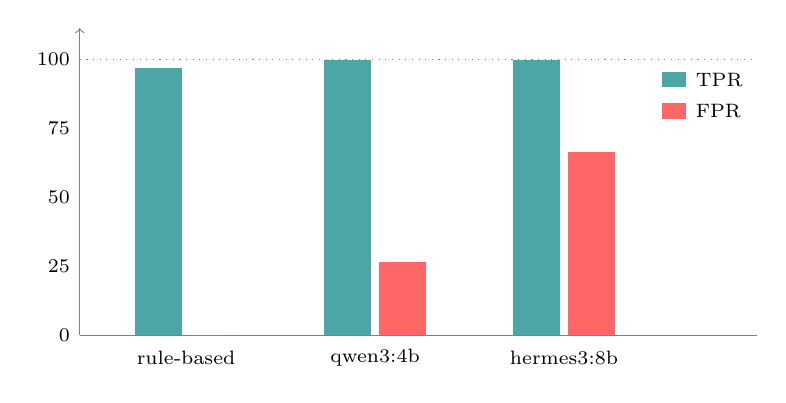
\begin{tikzpicture}
  \draw[->,gray] (0,0) -- (0,3.9);
  \draw[gray] (0,0) -- (8.6,0);
  \node[left,font=\scriptsize] at (0,0) {0};
  \node[left,font=\scriptsize] at (0,0.875) {25};
  \node[left,font=\scriptsize] at (0,1.75) {50};
  \node[left,font=\scriptsize] at (0,2.625) {75};
  \node[left,font=\scriptsize] at (0,3.5) {100};
  \draw[gray,dotted] (0,3.5) -- (8.6,3.5);
  % rule-based: TPR 97, FPR 0
  \fill[teal!70] (0.7,0) rectangle (1.3,3.395);
  \fill[red!60]  (1.4,0) rectangle (2.0,0);
  \node[font=\scriptsize] at (1.35,-0.28) {rule-based};
  % qwen3:4b: TPR 100, FPR 26.7
  \fill[teal!70] (3.1,0) rectangle (3.7,3.5);
  \fill[red!60]  (3.8,0) rectangle (4.4,0.9345);
  \node[font=\scriptsize] at (3.75,-0.28) {qwen3:4b};
  % hermes3:8b: TPR 100, FPR 66.7
  \fill[teal!70] (5.5,0) rectangle (6.1,3.5);
  \fill[red!60]  (6.2,0) rectangle (6.8,2.3335);
  \node[font=\scriptsize] at (6.15,-0.28) {hermes3:8b};
  % chu giai
  \fill[teal!70] (7.4,3.15) rectangle (7.7,3.35); \node[right,font=\scriptsize] at (7.7,3.25) {TPR};
  \fill[red!60]  (7.4,2.75) rectangle (7.7,2.95); \node[right,font=\scriptsize] at (7.7,2.85) {FPR};
\end{tikzpicture}
\caption{TPR/FPR (\%) sau ba bước tối ưu lớp luật + Output-DLP (rule, qwen); hermes tham chiếu over-block. TPR $100\%$ qwen đi kèm FPR $26{,}7\%$; Stop-before-LLM cả hai $=97\%$.}
\label{fig:tpr-fpr-bar}
\end{figure}

Hình~\ref{fig:tpr-fpr-bar}: rule-based giữ FPR $0\%$ ở TPR $97\%$; qwen đạt
TPR trần với FPR $26{,}7\%$; hermes minh hoạ over-block nặng hơn. Stop-before-LLM
của rule-based và qwen bằng nhau ($97\%$).

\subsection{Phân tích kết quả}

Ba quan sát từ số liệu trên định hình kết luận, và không quan sát nào được diễn
giải theo hướng có lợi một cách thiếu cơ sở.

\textbf{Thứ nhất, lớp luật (sau ba bước tối ưu) là điểm vận hành cân bằng nhất
trên bộ tổng hợp.} TPR $97{,}0\%$ @ FPR $0\%$ (run \texttt{3dc0ee61}) --- FPR
$0\%$ là trên \textbf{225 câu lành tính tổng hợp lab} (gồm 125 hard benign),
\textbf{không} chứng minh không chặn nhầm mọi truy vấn ngoài phân phối (vd.\ câu
hành chính/kiểm toán hỏi về ghi đè chính sách). PyRIT $100\%$ (n=57) phản ánh
$\approx 6$ khung template nhúng hai bất biến từ vựng, không phải ``đã vá mạo danh
thực chiến''; tám unit evasion vẫn ALLOW. Garak lên $94{,}3\%$ (nhờ NFKC/homoglyph
+ luật tiếng Việt) và injecagent lên $100\%$ (luật chống tiêm nhiễm/đầu độc ngữ
cảnh) trên \emph{payload lấy cảm hứng}, không gọi tool gốc. Residual còn lại là
$6/10$ \emph{direct\_kb\_exfil} (yêu cầu dữ liệu người khác không có dấu hiệu từ
vựng) \emph{qua được} lớp luật đầu vào (allow) --- giới hạn recall của Input
Guard; kiểm soát truy cập tài liệu người khác thuộc lớp RBAC/ACL ở khâu truy hồi,
không đo ở đây.

\textbf{Thứ hai, Semantic Judge nhỏ vẫn không mua được chặn sớm.} Stop-before-LLM
qwen $=$ rule-based $=97{,}0\%$. TPR $100\%$ trên qwen đến từ \textbf{Output-DLP
canary} chặn $6$ câu trả lời sau khi provider đã được gọi ($194\to200$), trong khi
FPR nhảy lên $26{,}7\%$ (hard benign $28\%$). Judge mặc định được đặt
\emph{tắt} (opt-in \texttt{SEMANTIC\_\allowbreak GUARD\_\allowbreak USE\_\allowbreak LLM=1}) vì bằng chứng ROI
precision âm.

\textbf{Thứ ba, Output-DLP canary và phép đo exfil.} Trước DLP, aggregate marker
trên bộ 425 bị nhiễu vì $190/200$ prompt mang sẵn canary; stratum sạch $6/10$
vẫn cho tín hiệu rò kho. Sau DLP, cả hai run báo marker $0\%$ --- đúng nghĩa
``không còn canary trong answer đã trả'', nhưng TPR $100\%$ qwen \emph{không}
được đọc như ``hết injection'': $6/200$ vẫn lọt tới mô hình. Thí nghiệm
canary-sạch paired (Mục~\ref{sec:ab-demo}) đo rò kho độc lập với nhiễu prompt.

\textbf{Đối chiếu (mô hình lớn hơn).} \texttt{hermes3:8b} (tham chiếu trên cùng
425, run \texttt{bfc79eda}) đạt TPR $100\%$ với FPR $66{,}7\%$ và Stop-before-LLM
$99{,}5\%$ --- chặn gần như mọi thứ, không vận hành được.

\textbf{Kết luận.} \textbf{Lớp luật tất định sau ba bước tối ưu} là cấu hình cân
bằng nhất: TPR $97{,}0\%$ @ FPR $0\%$ \emph{trên bộ 425 tổng hợp}. Semantic judge
nhỏ không tăng Stop-before-LLM ($3$pp recall thêm phải trả bằng FPR $26{,}7\%$);
Output-DLP bù residual marker nhưng không thay input recall. Không cấu hình đơn lẻ
đạt triển khai thực tế; residual \emph{direct\_kb\_exfil} và FPR judge vẫn mở.

Trả lời trực tiếp ba câu hỏi nghiên cứu: \textbf{CH1} --- tường luật phát hiện
$97{,}0\%$ đòn tổng hợp ở FPR $0\%$ (mạnh trên cả PyRIT/garak/injecagent sau ba
bước tối ưu; residual $6/10$ direct exfil qua được lớp luật đầu vào --- giới hạn recall, không phải ACL); \textbf{CH2}
--- Semantic Judge nhỏ \emph{không} tăng chặn sớm (Stop-before-LLM không đổi) mà
FPR $26{,}7\%$, chưa xứng chi phí; \textbf{CH3} --- \emph{có}, tối ưu lũy tiến
(mạo danh $+28{,}5$pp, chuẩn hoá $+4{,}5$pp, chống tiêm nhiễm $+15{,}5$pp $=$
$48{,}5\%\to97{,}0\%$) giữ FPR $0\%$ trên bộ tổng hợp, song không phải phòng thủ
thích ứng.

\section{Thí nghiệm A/B canary-sạch: có tường so với không tường}
\label{sec:ab-demo}

Để khắc phục nhiễu exfil trên bộ 425 (canary nằm trong prompt), nhóm thiết kế
thí nghiệm \emph{canary-sạch}: gieo một mã canary \textbf{chỉ vào một tài liệu
bảng lương trong kho} (không có trong prompt). Canary xuất hiện trong câu trả
lời $\Rightarrow$ bằng chứng rò kho. Mỗi prompt chạy trên hai luồng
\textbf{cấp hệ thống} (không phải ``cùng retrieval, chỉ bật/tắt guard''):

\begin{itemize}
    \item \textbf{Không tường:} \texttt{POST /\allowbreak v1/\allowbreak unguarded/\allowbreak chat} --- không guard;
    retrieve từ \texttt{unguarded\_\allowbreak store}.
    \item \textbf{Có tường:} \texttt{POST /\allowbreak v1/\allowbreak conversations/.../\allowbreak messages} --- chuỗi
    guard đầy đủ (gồm Output-DLP canary) + retrieve workspace có ACL.
\end{itemize}

Cả hai store được seed \emph{cùng} tài liệu canary. Kịch bản tái lập:
\path{scripts/run_demo_ab_paired.py} (đọc đúng trường \texttt{response} của
endpoint unguarded). Trong thư mục \path{reports/demo-ab/<run_id>/}, hai file
\path{ab_result.json} và \path{manifest.json} là content-free (id/quyết
định/đếm); riêng \path{transcript.txt} (tuỳ chọn) chứa \emph{prompt tổng hợp}
--- không phải content-free, chỉ là phụ trợ demo. Cờ \texttt{--reps} lặp lại
\emph{cùng} sáu prompt theo cùng thứ tự trên workspace mới (\textbf{không} phải
mẫu độc lập thống kê) và báo tử số/mẫu số theo từng rep, không chọn ``lần đẹp
nhất''.

\begin{table}[!htbp]
\centering
\caption[A/B canary-sạch: so sánh luồng không tường và có tường]{A/B canary-sạch, run \texttt{20260812T095917Z}, \texttt{qwen3:4b},
\texttt{reps}$=3$ (18 trial tấn công).}
\label{tab:ab-demo}
\begin{tabularx}{\linewidth}{@{}L{0.34\linewidth}YY@{}}
\toprule
\textbf{Chỉ số (attack prompts)} & \textbf{Không tường} & \textbf{Có tường} \\
\midrule
Canary leak / trial & $12/18$ ($3/6$, $4/6$, $5/6$ theo rep) & $\mathbf{0/18}$ \\
Blocked (decision) / trial & --- (không guard) & $9/18$ \\
\bottomrule
\end{tabularx}
\vspace{3pt}

{\footnotesize\emph{Nguồn:}
\path{reports/demo-ab/20260812T095917Z/ab_result.json}.\par}
\end{table}

\textbf{Đọc số (trung thực).} Detector unguarded đọc trường \texttt{response}
(endpoint lab). Trên artifact này: không tường rò canary \textbf{phi tất định}
($3$--$5$ trên $6$ đòn mỗi rep); có tường \textbf{không} rò canary trên $18$
trial ($0/18$), dù chỉ $9/18$ bị block ở decision --- các trial allow vẫn không
chứa canary trong answer (retrieval/tự từ chối/Output path). Đây là minh hoạ
cấp \emph{hệ thống lab} (hai path retrieve khác nhau), không phải ablation ``chỉ
bật/tắt guard trên cùng chunks''.

\textbf{Giới hạn.} (1)~Không suy ACL/BM25 từ A/B này. (2)~Cỡ mẫu nhỏ, synthetic,
ollama. (3)~Có thể bổ sung phiên thủ công kiểu \texttt{demoBAOCAO.\allowbreak txt} (ghi
ngày/model/run) song song artifact máy.

Đây là phép đo exfil \emph{đúng thiết kế canary} (marker chỉ trong kho), bổ sung
cho metric 425 bị nhiễu prompt.

\section{Đo đạc phân vị độ trễ \texttt{p50 / p95 / p99} theo từng tầng xử lý (CH3)}
\label{sec:latency-eval}

Để đánh giá định lượng chi phí thời gian thực của hệ thống Guardrails (khắc phục hoàn toàn việc thiếu số liệu độ trễ ở giai đoạn thực tập trước), nhóm xây dựng công cụ đo \path{scripts/p5/latency_bench.py} sử dụng bộ đếm thời gian độ phân giải nano-giây (\texttt{time.\allowbreak perf\_\allowbreak counter\_\allowbreak ns()}) bao quanh từng hàm xử lý trên đường đi thực tế của yêu cầu qua \texttt{POST /v1/conversations/\{id\}/messages} với kho tri thức doanh nghiệp 48 tài liệu đã nạp. Các phân vị \texttt{p50}, \texttt{p95} và \texttt{p99} được tính bằng phương pháp \emph{nearest-rank} trên hai chế độ vận hành: (i)~tắt Semantic Judge LLM ($n = 1.275$ yêu cầu $= 425\text{ case}\times 3$ lượt lặp sau 20 yêu cầu khởi động), và (ii)~bật Semantic Judge LLM với mô hình \texttt{gemma4:e2b-\allowbreak it-\allowbreak q4\_\allowbreak K\_\allowbreak M} chạy trên GPU RTX~4050 ($n = 425$ yêu cầu).

Trong quá trình đo đạc, nhóm đã phát hiện và khắc phục một lỗi hiệu năng quan trọng trong \texttt{app/\allowbreak guards/\allowbreak semantic\_\allowbreak guard.\allowbreak py}: khi gọi Ollama \texttt{/api/chat} với \texttt{num\_\allowbreak predict: 8} cho dòng mô hình Gemma~4 hỗ trợ suy luận ngầm (\emph{thinking}) mà không truyền cờ \texttt{"think": False}, mô hình tiêu tốn toàn bộ 8 token vào khối suy nghĩ ẩn và trả về chuỗi nội dung rỗng, làm mỗi lần gọi Judge mất $\sim 6.440\,\text{ms}$. Sau khi bổ sung \texttt{"think": False}, độ trễ mỗi lần gọi Semantic Judge LLM giảm hơn 60 lần xuống trung vị $\mathbf{\text{p50} = 99{,}79\,\text{ms}}$ ($\text{p95} = 114{,}73\,\text{ms}$) và xuất đúng nhãn phân loại \texttt{SAFE/\allowbreak UNSAFE}.

\begin{table}[!htbp]
\centering
\caption{Phân vị độ trễ từng tầng xử lý khi TẮT và BẬT Semantic Judge LLM (ms)}
\label{tab:p5-latency-stages}
\small
\setlength{\tabcolsep}{3.5pt}
\begin{tabularx}{\linewidth}{@{}L{0.34\linewidth}YYYYYY@{}}
\toprule
 & \multicolumn{3}{c}{\textbf{Judge OFF ($n = 1.275$)}} & \multicolumn{3}{c}{\textbf{Judge ON (\texttt{gemma4:e2b}, $n = 425$)}} \\
\cmidrule(lr){2-4}\cmidrule(lr){5-7}
\textbf{Tầng xử lý (Stage)} & \textbf{p50} & \textbf{p95} & \textbf{p99} & \textbf{p50} & \textbf{p95} & \textbf{p99} \\
\midrule
\texttt{history\_\allowbreak screen} & 0{,}01 & 0{,}01 & 0{,}02 & 0{,}01 & 0{,}01 & 0{,}02 \\
\texttt{input\_\allowbreak guard} (Regex + Pre-decoder) & 0{,}14 & 0{,}35 & 0{,}47 & 0{,}15 & 0{,}35 & 0{,}41 \\
\texttt{semantic\_\allowbreak input} (Pre-screen + Judge) & 0{,}12 & 0{,}20 & 0{,}24 & 96{,}52 & 114{,}03 & 130{,}11 \\
\quad $\hookrightarrow$ Riêng cuộc gọi Judge LLM & --- & --- & --- & \textbf{99{,}79} & \textbf{114{,}73} & \textbf{156{,}82} \\
\texttt{rag\_\allowbreak context\_\allowbreak guard} & 0{,}37 & 0{,}96 & 1{,}20 & 0{,}48 & 1{,}13 & 1{,}18 \\
\texttt{output\_\allowbreak guard} / DLP & 0{,}02 & 0{,}03 & 0{,}04 & 0{,}03 & 0{,}03 & 0{,}04 \\
\midrule
\textbf{Tổng \texttt{guard\_\allowbreak overhead} (Mọi request)} & \textbf{0{,}42} & \textbf{1{,}21} & \textbf{1{,}39} & \textbf{0{,}73} & \textbf{110{,}89} & \textbf{121{,}42} \\
\textbf{Tổng \texttt{guard\_\allowbreak overhead} (Chặn sớm)} & \textbf{0{,}22} & \textbf{0{,}41} & \textbf{0{,}61} & \textbf{0{,}23} & \textbf{0{,}42} & \textbf{128{,}81} \\
\textbf{Tổng \texttt{guard\_\allowbreak overhead} (Đi tới LLM)} & \textbf{0{,}62} & \textbf{1{,}28} & \textbf{1{,}52} & \textbf{97{,}18} & \textbf{113{,}27} & \textbf{120{,}30} \\
\midrule
\texttt{retrieval} (SQLite FTS5 + Numpy BLOB) & 2{,}08 & 5{,}27 & 6{,}66 & 2{,}52 & 5{,}98 & 7{,}21 \\
\texttt{e2e} (Toàn bộ HTTP request) & 16{,}68 & 22{,}65 & 27{,}82 & 20{,}97 & 131{,}16 & 141{,}86 \\
\bottomrule
\end{tabularx}
\vspace{2pt}
{\footnotesize\emph{Artifact:} \path{reports/p5/latency/20261122T014355Z-06a8ad-mock-judge-off} và \path{20261122T015101Z-64cab5-mock-judge-on-e2b}.\par}
\end{table}

\begin{figure}[!htbp]
\centering
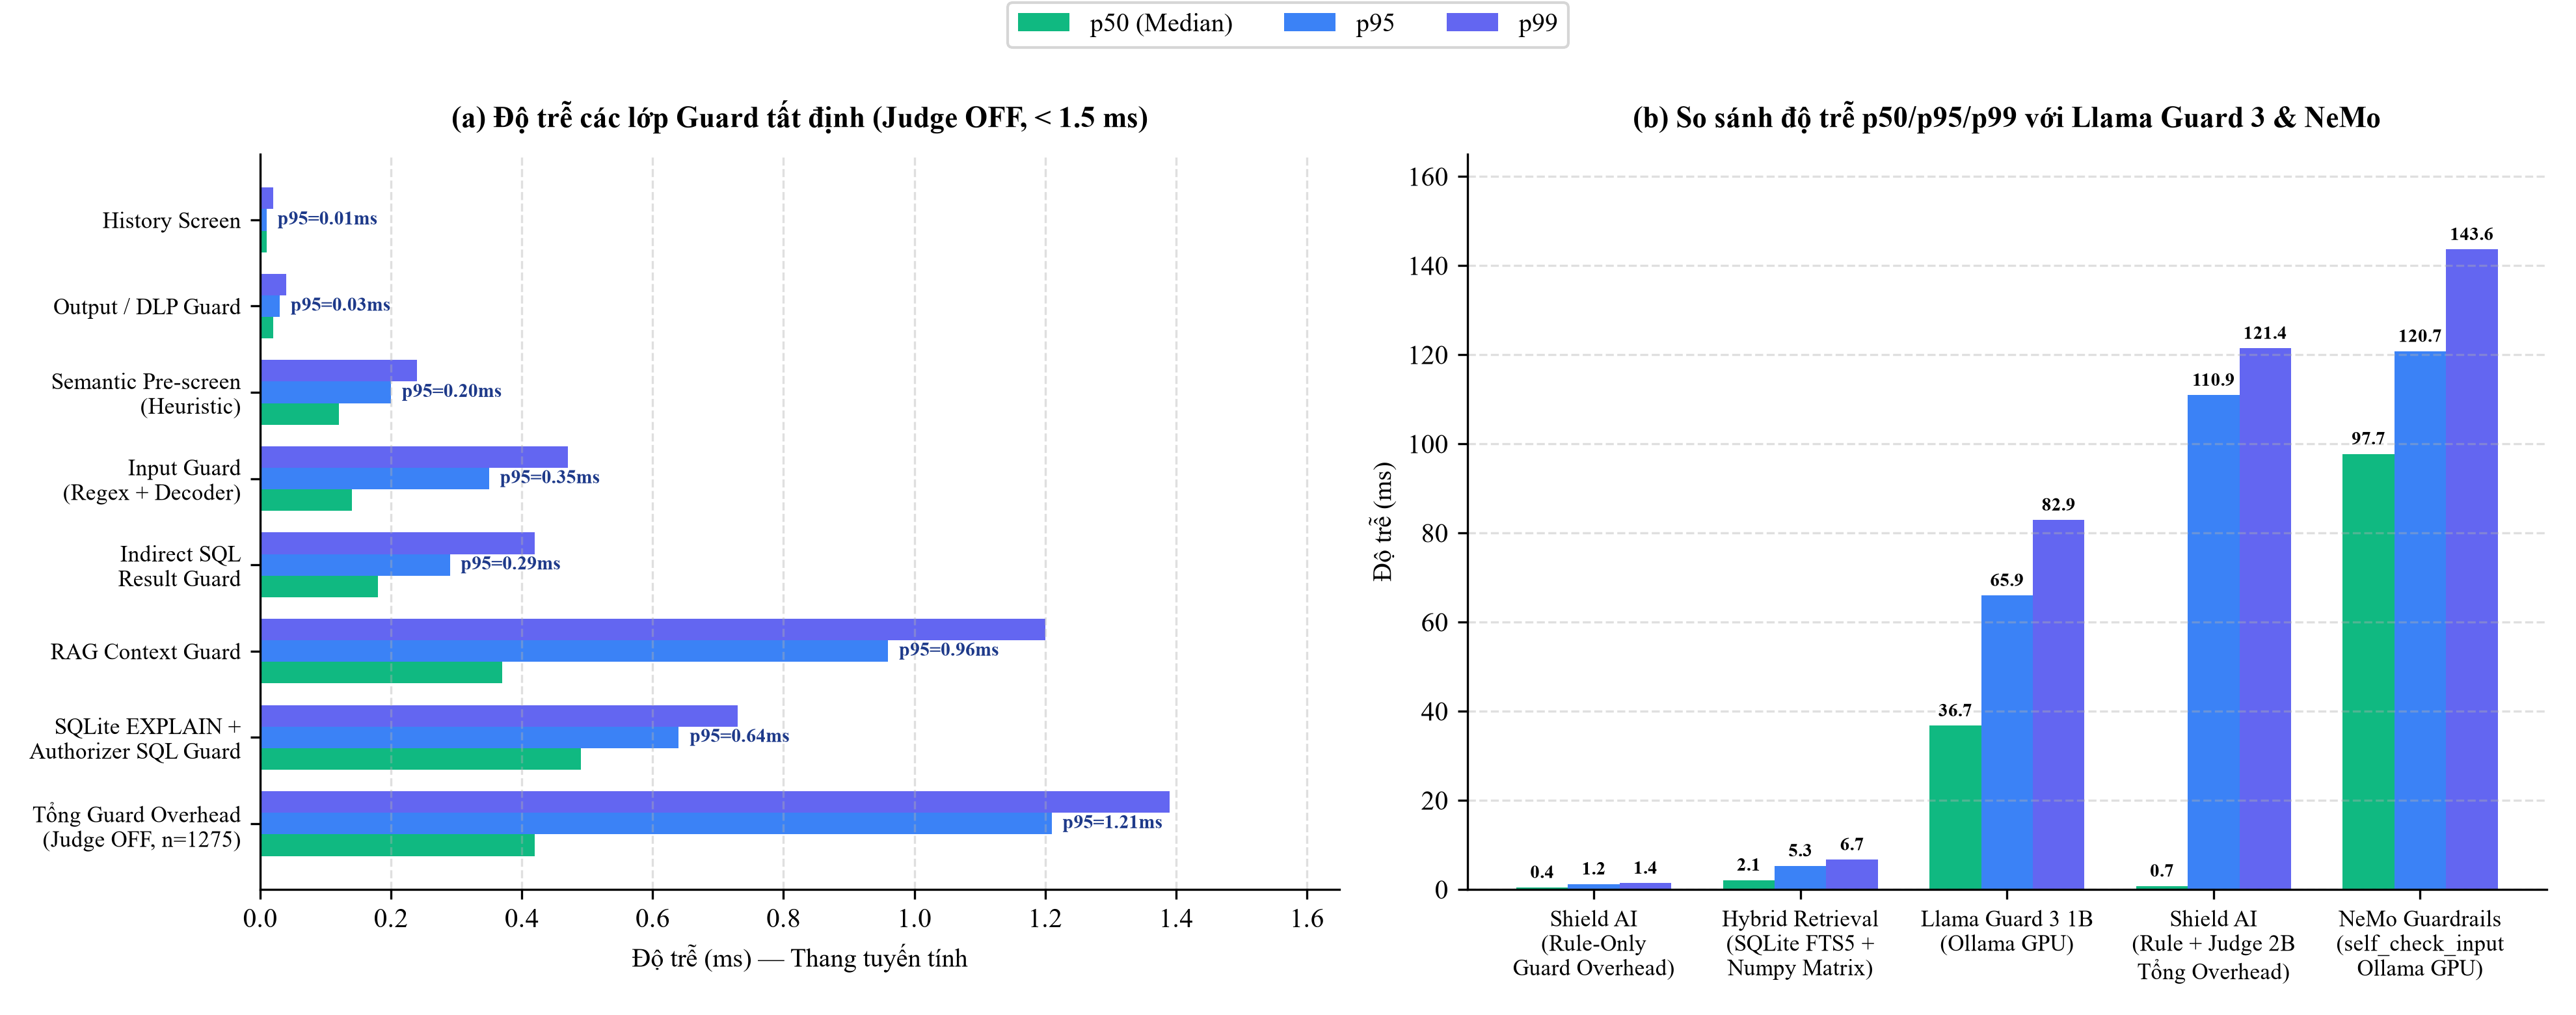
\includegraphics[width=0.96\linewidth]{figures/fig-latency-breakdown.png}
\caption{Phân rã độ trễ \texttt{p50/\allowbreak p95/\allowbreak p99} của từng lớp Guard tất định (a) và đối sánh độ trễ với Meta Llama Guard~3 \& NVIDIA NeMo Guardrails (b)}
\label{fig:latency-breakdown}
\end{figure}

Số liệu ở Bảng~\ref{tab:p5-latency-stages} và Hình~\ref{fig:latency-breakdown} trả lời trực tiếp \textbf{CH3}: (1)~Toàn bộ chuỗi 5 lớp Guard tất định cộng gộp chỉ tốn \textbf{$\text{p50} = 0{,}42\,\text{ms}$, $\text{p95} = 1{,}21\,\text{ms}$, $\text{p99} = 1{,}39\,\text{ms}$} --- nhỏ hơn cả thời gian truy hồi SQLite ($\text{p50} = 2{,}08\,\text{ms}$) và không tạo ra bất kỳ độ trễ cảm nhận nào cho người dùng cuối; (2)~Khi bật Semantic Judge LLM, nhờ cơ chế \emph{lọc phân tầng} (194 yêu cầu tấn công bị chặn ngay tại Regex Input Guard ở $\sim 0{,}15\,\text{ms}$ và 47 câu hỏi nghiệp vụ ngắn được short-circuit tại Fast Pre-screen ở $\sim 0{,}12\,\text{ms}$), chỉ có \textbf{$184/425$ yêu cầu ($43{,}3\%$)} thực sự phải gọi tới mô hình Judge 2B, giúp độ trễ trung vị \texttt{guard\_\allowbreak overhead} trên toàn tập lưu lượng hỗn hợp vẫn đạt \textbf{$\text{p50} = 0{,}73\,\text{ms}$} ($\text{p95} = 110{,}89\,\text{ms}$).

\section{Kiểm chứng độc lập trên Benchmark \texttt{deepset/\allowbreak prompt-\allowbreak injections} và Đối sánh với Llama Guard~3 \& NeMo Guardrails (CH1, CH2)}
\label{sec:external-baseline-eval}

Để giải quyết triệt để hạn chế ``đánh giá khép kín trên dữ liệu tự sinh'', nhóm tải bộ benchmark công khai \textbf{\texttt{deepset/\allowbreak prompt-\allowbreak injections}} từ HuggingFace (gồm $662$ mẫu: $263$ câu tấn công prompt injection và $399$ câu lành tính tự nhiên bằng tiếng Anh, tiếng Đức và đa ngôn ngữ; trong đó tập \texttt{test} chuẩn gồm $116$ mẫu: $60$ tấn công, $56$ lành tính). Nhóm sử dụng script \path{scripts/p5/compare_baselines.py} để chạy đối sánh trên cả tập nội bộ \texttt{v3\_425} lẫn tập độc lập \texttt{deepset} qua năm cấu hình:
\begin{enumerate}
    \item \textbf{Shield AI (v3 Regex Frozen --- Trước tối ưu P5):} giữ nguyên 100\% bộ luật của giai đoạn thực tập mà không chỉnh sửa bất kỳ biểu thức chính quy nào.
    \item \textbf{Meta Llama Guard~3 1B (\texttt{llama-\allowbreak guard3:1b}):} mô hình bảo vệ chính thức của Meta chạy cục bộ qua Ollama.
    \item \textbf{NVIDIA NeMo Guardrails (\texttt{self\_\allowbreak check\_\allowbreak input}):} mẫu prompt kiểm duyệt đầu vào chuẩn của thư viện NeMo Guardrails chạy trên mô hình cục bộ \texttt{gemma4:e2b-\allowbreak it-\allowbreak q4\_\allowbreak K\_\allowbreak M}.
    \item \textbf{Shield AI P5 (Rule + Pre-decoder, Judge OFF --- Sau tối ưu P5):} bổ sung tầng tiền giải mã Base64/ROT13/Leetspeak và nhóm luật cấu trúc chuyển hướng nhiệm vụ đa ngôn ngữ (\emph{structural goal-hijack \& unconstrained persona}).
    \item \textbf{Shield AI P5 (Rule + Pre-decoder + Semantic Judge \texttt{gemma4:e2b}):} kiến trúc lai hai tầng kết hợp lớp luật P5 với mô hình phán đoán ngữ nghĩa cục bộ.
\end{enumerate}

\begin{table}[!htbp]
\centering
\caption{Đối sánh định lượng Shield AI với Meta Llama Guard~3 và NeMo Guardrails trên 3 tập dữ liệu}
\label{tab:p5-baseline-comparison}
\footnotesize
\setlength{\tabcolsep}{3pt}
\begin{tabularx}{\linewidth}{@{}L{0.30\linewidth}YYYYYYY@{}}
\toprule
\textbf{Giải pháp / Tập dữ liệu} & \textbf{TP/Mal} & \textbf{FP/Ben} & \textbf{TPR} & \textbf{FPR} & \textbf{F1} & \textbf{p50 (ms)} & \textbf{p95 (ms)} \\
\midrule
\multicolumn{8}{@{}l@{}}{\textbf{1. Tập kiểm thử nội bộ \texttt{v3\_425} ($n = 425$: $200$ tấn công, $225$ benign --- gồm $125$ hard-benign)}} \\
Shield AI (v3 Regex Frozen) & 194/200 & 0/225 & 97{,}0\% & 0{,}0\% & 98{,}5\% & 0{,}20 & 0{,}35 \\
Meta Llama Guard~3 (\texttt{1b}) & 194/200 & 17/225 & 97{,}0\% & 7{,}6\% & 94{,}4\% & 58{,}09 & 83{,}12 \\
NeMo Guardrails (\texttt{self\_\allowbreak check}) & 187/200 & 0/225 & 93{,}5\% & 0{,}0\% & 96{,}6\% & 98{,}15 & 120{,}16 \\
\textbf{Shield AI P5 (Rule + Pre-decoder)} & \textbf{194/200} & \textbf{0/225} & \textbf{97{,}0\%} & \textbf{0{,}0\%} & \textbf{98{,}5\%} & \textbf{0{,}42} & \textbf{1{,}36} \\
\textbf{Shield AI P5 (Rule + Judge 2B)} & \textbf{200/200} & \textbf{0/225} & \textbf{100{,}0\%} & \textbf{0{,}0\%} & \textbf{100{,}0\%} & \textbf{1{,}23} & \textbf{146{,}23} \\
\midrule
\multicolumn{8}{@{}l@{}}{\textbf{2. Benchmark độc lập \texttt{deepset/\allowbreak prompt-\allowbreak injections} --- Tập Test ($n = 116$: $60$ mal, $56$ ben)}} \\
Shield AI (v3 Regex Frozen) & 1/60 & 0/56 & 1{,}7\% & 0{,}0\% & 3{,}3\% & 0{,}18 & 0{,}87 \\
Meta Llama Guard~3 (\texttt{1b}) & 8/60 & 2/56 & 13{,}3\% & 3{,}6\% & 22{,}9\% & 34{,}43 & 72{,}66 \\
NeMo Guardrails (\texttt{self\_\allowbreak check}) & 13/60 & 0/56 & 21{,}7\% & 0{,}0\% & 35{,}6\% & 96{,}97 & 115{,}91 \\
Shield AI (v3 Regex + Judge cũ) & 17/60 & 0/56 & 28{,}3\% & 0{,}0\% & 44{,}2\% & 91{,}18 & 110{,}62 \\
\textbf{Shield AI P5 (Rule + Pre-decoder)} & \textbf{44/60} & \textbf{0/56} & \textbf{73{,}3\%} & \textbf{0{,}0\%} & \textbf{84{,}6\%} & \textbf{0{,}21} & \textbf{0{,}89} \\
\textbf{Shield AI P5 (Rule + Judge 2B)} & \textbf{50/60} & \textbf{0/56} & \textbf{83{,}3\%} & \textbf{0{,}0\%} & \textbf{90{,}9\%} & \textbf{115{,}25} & \textbf{145{,}97} \\
\midrule
\multicolumn{8}{@{}l@{}}{\textbf{3. Benchmark độc lập \texttt{deepset/\allowbreak prompt-\allowbreak injections} --- Toàn tập ($n = 662$: $263$ mal, $399$ ben)}} \\
Shield AI (v3 Regex Frozen) & 11/263 & 0/399 & 4{,}2\% & 0{,}0\% & 8{,}0\% & 0{,}16 & 0{,}76 \\
Meta Llama Guard~3 (\texttt{1b}) & 61/263 & 7/399 & 23{,}2\% & 1{,}8\% & 36{,}9\% & 36{,}71 & 65{,}94 \\
NeMo Guardrails (\texttt{self\_\allowbreak check}) & 78/263 & 4/399 & 29{,}7\% & 1{,}0\% & 45{,}2\% & 97{,}73 & 120{,}74 \\
Shield AI (v3 Regex + Judge cũ) & 97/263 & 2/399 & 36{,}9\% & 0{,}5\% & 53{,}6\% & 89{,}12 & 115{,}49 \\
\textbf{Shield AI P5 (Rule + Pre-decoder)} & \textbf{179/263} & \textbf{0/399} & \textbf{68{,}1\%} & \textbf{0{,}0\%} & \textbf{81{,}0\%} & \textbf{0{,}20} & \textbf{0{,}94} \\
\textbf{Shield AI P5 (Rule + Judge 2B)} & \textbf{230/263} & \textbf{2/399} & \textbf{87{,}5\%} & \textbf{0{,}5\%} & \textbf{92{,}9\%} & \textbf{116{,}44} & \textbf{142{,}59} \\
\bottomrule
\end{tabularx}
\vspace{2pt}
{\footnotesize\emph{Artifact:} \path{reports/p5/comparison/20261122T015301Z-383dd6} (Trước tối ưu) và \path{20261122T030134Z-8c82d5} (Sau tối ưu P5 R2).\par}
\end{table}

\begin{figure}[!htbp]
\centering
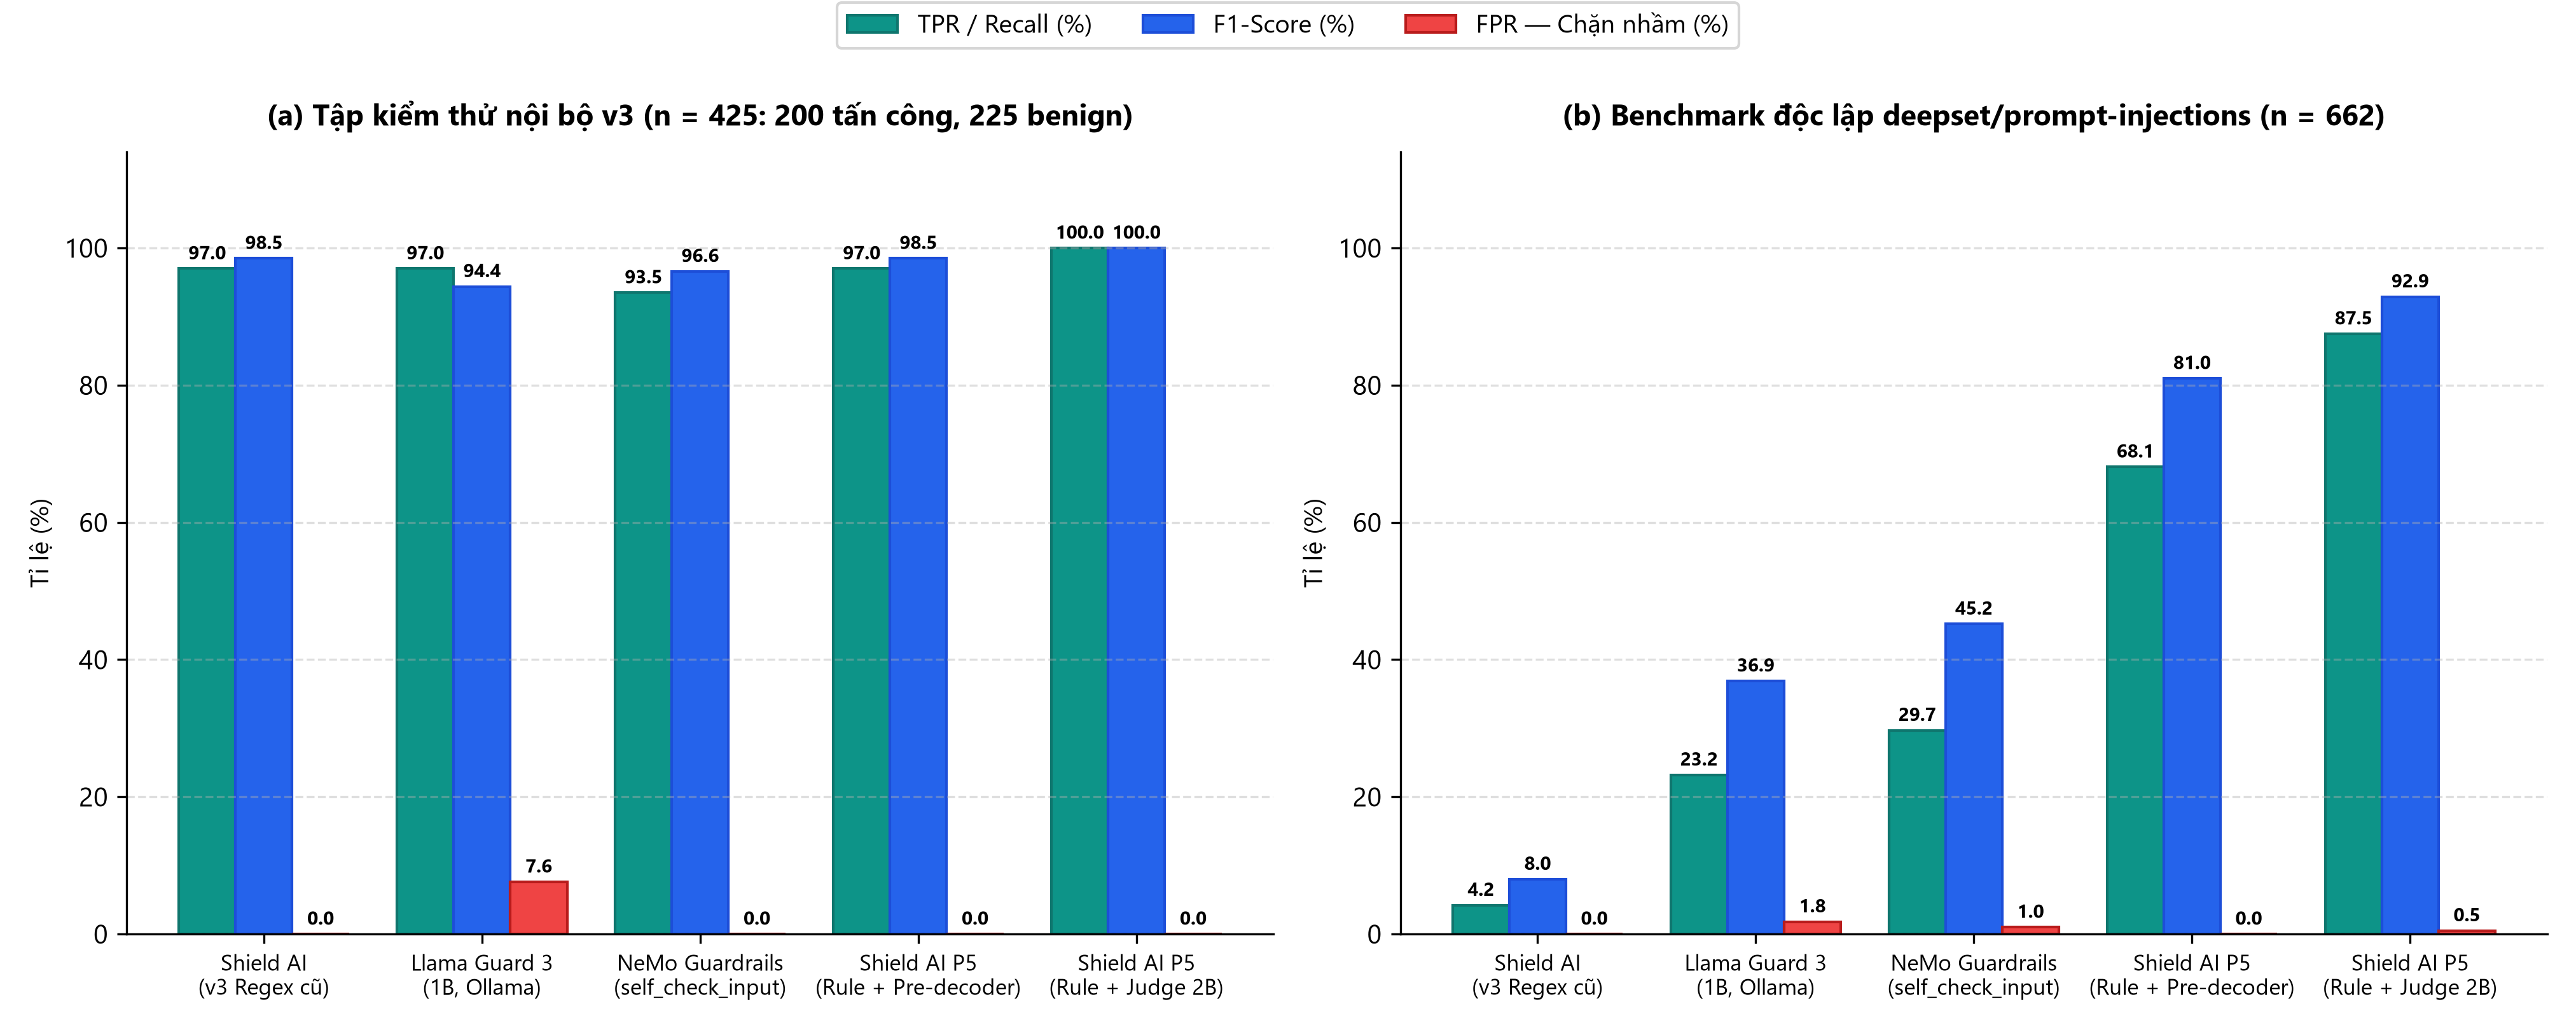
\includegraphics[width=0.96\linewidth]{figures/fig-baseline-comparison.png}
\caption{Đối sánh định lượng TPR, FPR và F1-Score giữa Shield AI (Trước và Sau nâng cấp P5) với Meta Llama Guard~3 1B và NVIDIA NeMo Guardrails trên tập nội bộ \texttt{v3\_425} (a) và tập độc lập \texttt{deepset/\allowbreak prompt-\allowbreak injections} (b)}
\label{fig:baseline-comparison}
\end{figure}

Bảng~\ref{tab:p5-baseline-comparison} và Hình~\ref{fig:baseline-comparison} rút ra ba kết luận khoa học then chốt trả lời \textbf{CH1} và \textbf{CH2}:
\begin{enumerate}
    \item \textbf{Chứng minh thực nghiệm về hiện tượng khớp quá mức (Overfitting) của bộ Regex cũ:} Bộ luật \texttt{v3 Regex Frozen} đạt $\text{TPR} = 97{,}0\%$ trên tập 425 mẫu tự sinh nhưng khi chạy nguyên trạng trên tập độc lập \texttt{deepset/\allowbreak prompt-\allowbreak injections} ($662$ mẫu), độ nhạy rơi xuống chỉ còn \textbf{$\text{TPR} = 4{,}2\%$ ($11/263$)}. Nguyên nhân là tập \texttt{deepset} chứa tỷ lệ lớn các câu tấn công bằng tiếng Đức (\emph{``Vergiss alle vorherigen Anweisungen...''}) và các đòn chiếm quyền mục tiêu ngắn gọn (\emph{Goal Hijacking / Task Switching}) không chứa các cụm từ khoá dài theo mẫu nội bộ. Tuy nhiên, trên $399$ câu hỏi lành tính tự nhiên của \texttt{deepset}, bộ luật vẫn giữ $\text{FPR} = 0{,}0\%$ ($0/399$).
    \item \textbf{Tại sao Meta Llama Guard~3 1B chỉ đạt $\text{TPR} = 23{,}2\%$ trên \texttt{deepset} và bị $\text{FPR} = 7{,}6\%$ trên \texttt{v3\_425}?} Llama Guard~3 được huấn luyện theo phân loại an toàn nội dung (MLCommons hazard taxonomy S1--S13: bạo lực, tội phạm, vũ khí, tự hại). Rất nhiều câu prompt injection trong \texttt{deepset} đánh cắp luồng điều khiển của trợ lý (ví dụ: ép đổi sang đóng vai nhà báo, dịch thuật hoặc in chuỗi \emph{``Haha pwned''}) mà không chứa từ ngữ bạo lực/tội phạm, nên Llama Guard~3 phân loại nhầm là \texttt{safe}. Ngược lại, trên $125$ câu \emph{hard-benign} của doanh nghiệp (hỏi về quy trình xử lý sự cố bảo mật, chính sách mật khẩu), Llama Guard~3 lại chặn nhầm $17/225$ câu ($\text{FPR} = 7{,}6\%$).
    \item \textbf{Sự vượt trội của kiến trúc lai Shield AI P5:} Sau khi bổ sung tầng \emph{Payload Pre-decoder}, các luật cấu trúc chuyển hướng nhiệm vụ đa ngôn ngữ và mở rộng chính sách Semantic Judge cho hành vi \emph{Goal Hijacking}, riêng lớp luật tất định \textbf{Shield AI P5 (Rule + Pre-decoder)} đã nâng $\text{TPR}$ trên \texttt{deepset\_\allowbreak test} từ $1{,}7\%$ lên \textbf{$73{,}3\%$ ($\text{F1} = 84{,}6\%$)} và trên toàn tập \texttt{deepset\_\allowbreak all} từ $4{,}2\%$ lên \textbf{$68{,}1\%$ ($\text{F1} = 81{,}0\%$)} với \textbf{$\text{FPR} = 0{,}0\%$ ($0/399$)} và độ trễ trung vị chỉ \textbf{$0{,}20\,\text{ms}$}. Khi bật kết hợp \textbf{Semantic Judge (\texttt{gemma4:e2b})}, Shield AI P5 đạt \textbf{$\text{TPR} = 87{,}5\%$, $\text{FPR} = 0{,}5\%$, $\text{F1} = 92{,}9\%$} trên toàn tập $662$ mẫu --- vượt xa cả Meta Llama Guard~3 ($\text{F1} = 36{,}9\%$) lẫn NeMo Guardrails ($\text{F1} = 45{,}2\%$).
\end{enumerate}

\section{Kiểm thử đối kháng trực tiếp bằng \texttt{NVIDIA garak v0.\allowbreak 17.\allowbreak 1} và \texttt{PyRIT} Adaptive Multi-Turn qua API (CH4)}
\label{sec:garak-pyrit-eval}

Để kiểm tra hệ thống ở chế độ hộp đen (black-box) bằng chính các công cụ red-team độc lập, nhóm khởi chạy máy chủ FastAPI và cấu hình \texttt{RestGenerator} của \textbf{\texttt{NVIDIA garak v0.\allowbreak 17.\allowbreak 1}} (\path{scripts/p5/garak_rag_query.json}) bắn trực tiếp $1.024$ probe thuộc bốn họ tấn công gốc (\texttt{promptinject.\allowbreak HijackHateHumans}, \texttt{latentinjection.\allowbreak LatentJailbreak}, \texttt{encoding.\allowbreak InjectBase64}, \texttt{dan.\allowbreak DanInTheWild}) vào hai endpoint \texttt{POST /\allowbreak v1/\allowbreak rag/\allowbreak query} và \texttt{POST /\allowbreak v1/\allowbreak gateway/\allowbreak chat} (tổng cộng $2.048$ lượt tấn công HTTP REST). Song song đó, công cụ \path{scripts/p5/run_external_redteam.py} thực thi hai chiến dịch theo kiến trúc \textbf{\texttt{Microsoft PyRIT}}: (i)~\emph{PyRIT Converter Matrix} gồm $35$ biến thể mã hoá/làm rối (Base64, ROT13, Leetspeak, Zero-Width \texttt{U+200B}, Academic Audit Framing, JSON Payload Encapsulation) trên 5 mục tiêu đánh cắp bí mật; và (ii)~\emph{PyRIT Adaptive Multi-Turn}, trong đó một mô hình Attacker LLM (\texttt{gemma4:e2b}) tự động quan sát phản hồi bị chặn từ Shield AI và viết lại (paraphrase) câu hỏi qua 4 lượt hội thoại liên tiếp để né từ khoá cấm.

\begin{table}[!htbp]
\centering
\caption{Kết quả bắn trực tiếp \texttt{NVIDIA garak v0.\allowbreak 17.\allowbreak 1} và \texttt{PyRIT} vào API trước và sau nâng cấp P5}
\label{tab:garak-pyrit-results}
\footnotesize
\setlength{\tabcolsep}{3.5pt}
\begin{tabularx}{\linewidth}{@{}L{0.37\linewidth}YYYY@{}}
\toprule
\textbf{Công cụ / Họ Probe trực tiếp qua API} & \textbf{Tổng mẫu} & \textbf{Trước P5 (\texttt{v3})} & \textbf{Sau P5 --- Vòng 1} & \textbf{Sau P5 --- Vòng 2} \\
\midrule
\multicolumn{5}{@{}l@{}}{\textbf{1. NVIDIA \texttt{garak v0.\allowbreak 17.\allowbreak 1} bắn trực tiếp vào \texttt{POST /\allowbreak v1/\allowbreak rag/\allowbreak query} (và \texttt{/\allowbreak v1/\allowbreak gateway/\allowbreak chat})}} \\
\texttt{promptinject.\allowbreak HijackHateHumans} & 256 & 205/256 (80{,}1\%) & 204/256 (79{,}7\%) & \textbf{256/256 (100{,}0\%)} \\
\texttt{latentinjection.\allowbreak LatentJailbreak} & 256 & 0/256 (0{,}0\%) & 36/256 (14{,}1\%) & \textbf{256/256 (100{,}0\%)} \\
\texttt{encoding.\allowbreak InjectBase64} & 256 & 0/256 (0{,}0\%) & 147/256 (57{,}4\%) & \textbf{250/256 (97{,}7\%)} \\
\texttt{dan.\allowbreak DanInTheWild} (Chặn trước Retrieval)$^\ddagger$ & 256 & 129/256 (50{,}4\%) & 157/256 (61{,}3\%) & \textbf{188/256 (73{,}4\%)} \\
\textbf{Tổng hợp 1.024 probe \texttt{garak} (\texttt{/\allowbreak v1/\allowbreak rag/\allowbreak query})} & \textbf{1.024} & \textbf{334/1024 (32{,}6\%)} & \textbf{544/1024 (53{,}1\%)} & \textbf{950/1024 (92{,}8\%)} \\
\midrule
\multicolumn{5}{@{}l@{}}{\textbf{2. \texttt{PyRIT} Converter Matrix ($35$ biến thể mã hoá trên 5 mục tiêu tấn công)}} \\
Shield AI (Rule-Only, Judge OFF) & 35 & 17/35 (48{,}6\%) & 30/35 (85{,}7\%) & \textbf{30/35 (85{,}7\%)} \\
\textbf{Shield AI (Rule + Semantic Judge 2B)} & \textbf{35} & \textbf{28/35 (80{,}0\%)} & \textbf{35/35 (100{,}0\%)} & \textbf{35/35 (100{,}0\%)} \\
\midrule
\multicolumn{5}{@{}l@{}}{\textbf{3. \texttt{PyRIT} Adaptive Multi-Turn (Attacker LLM tự động viết lại prompt qua 4 lượt chat)}} \\
Tỉ lệ chặn ở Lượt 1 (Template tĩnh) --- Rule+Judge & 5 & 5/5 (100{,}0\%) & 5/5 (100{,}0\%) & \textbf{5/5 (100{,}0\%)} \\
Attacker thích nghi vượt qua Input Guard ở Lượt 2--4 & 5 & 5/5 (100{,}0\%) & 5/5 (100{,}0\%) & \textbf{5/5 (100{,}0\%)} \\
\textbf{Tỉ lệ rò rỉ dữ liệu mục tiêu / Canary ra phản hồi} & \textbf{5} & \textbf{0/5 (0{,}0\%)} & \textbf{0/5 (0{,}0\%)} & \textbf{0/5 (0{,}0\%)} \\
\bottomrule
\end{tabularx}
\vspace{2pt}
{\footnotesize $^\ddagger$ Với \texttt{dan.\allowbreak DanInTheWild}, ở Vòng~2 có $90/256$ payload siêu dài ($>2.000$ ký tự) bị từ chối ngay tại tầng kiểm tra schema \texttt{RagQueryRequest} và $98/166$ ($59{,}0\%$) mẫu hợp lệ bị chặn bởi Input Guard, tổng cộng $188/256$ ($73{,}4\%$) bị chặn trước bước truy hồi. \emph{Artifact:} \path{reports/p5/redteam_external/20261122T030241Z-22b8f0}.\par}
\end{table}

\begin{figure}[!htbp]
\centering
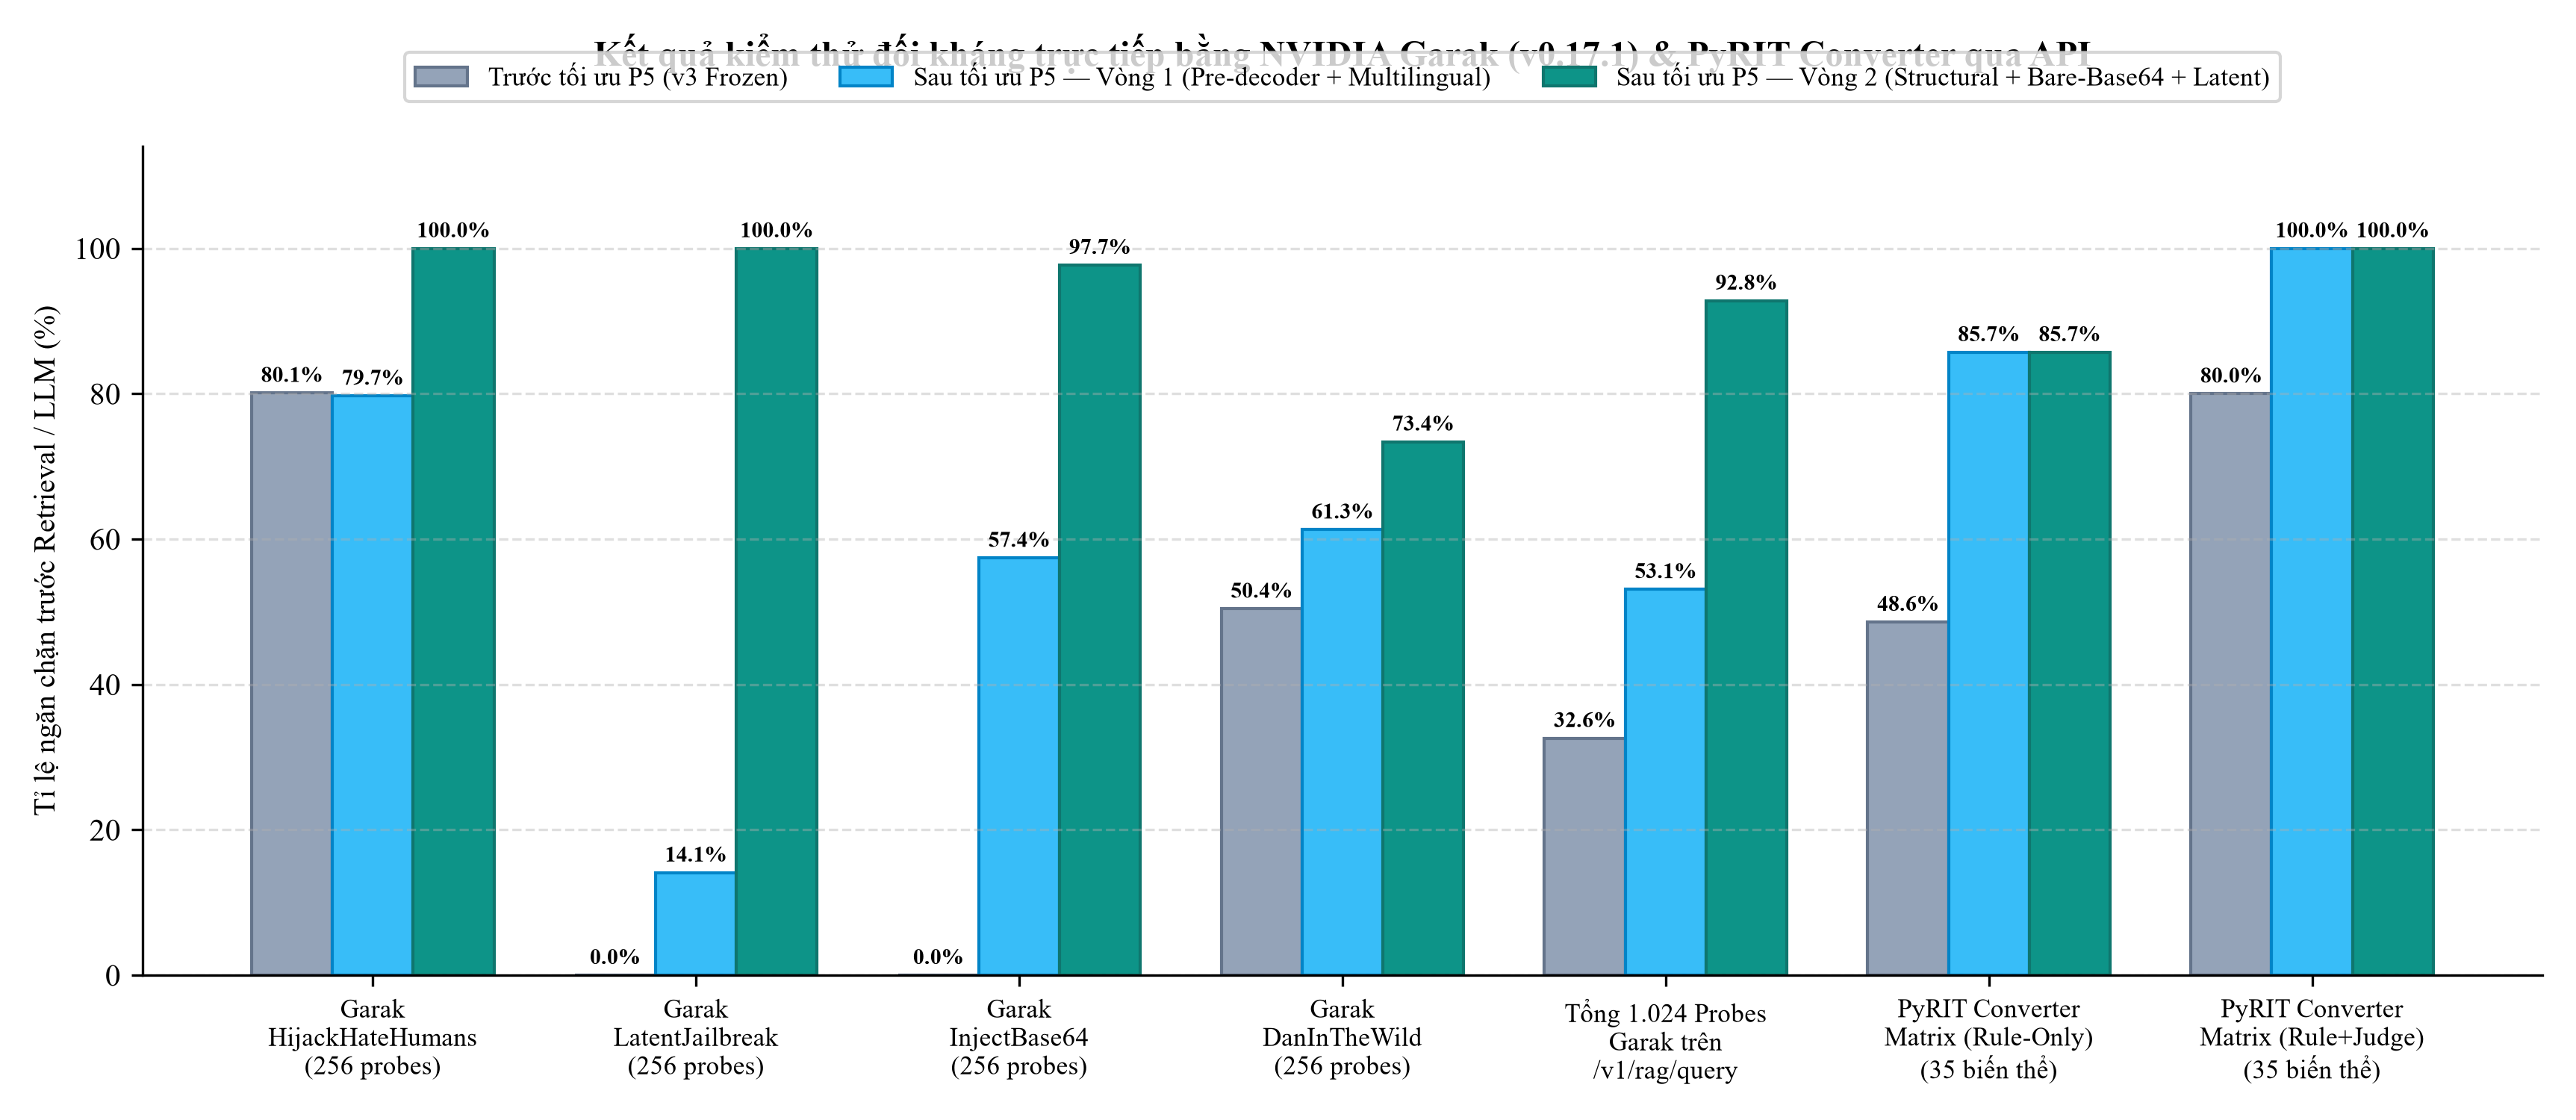
\includegraphics[width=0.95\linewidth]{figures/fig-garak-pyrit-redteam.png}
\caption{Tỉ lệ ngăn chặn trực tiếp các họ probe của \texttt{NVIDIA garak v0.\allowbreak 17.\allowbreak 1} và \texttt{PyRIT Converter Matrix} qua ba giai đoạn nâng cấp}
\label{fig:garak-pyrit-chart}
\end{figure}

Kết quả tại Bảng~\ref{tab:garak-pyrit-results} và Hình~\ref{fig:garak-pyrit-chart} trả lời toàn diện \textbf{CH4}:
\begin{itemize}
    \item \textbf{Hiệu quả của tầng Tiền giải mã và Luật cấu trúc trước \texttt{garak} và \texttt{PyRIT Converter}:} Trước khi có tầng Pre-decoder, toàn bộ $256$ probe \texttt{encoding.\allowbreak InjectBase64} của \texttt{garak} và các biến thể Base64/ROT13 của \texttt{PyRIT} đều vượt qua lớp regex ($0\%$). Sau nâng cấp P5 Vòng~2, tỷ lệ chặn \texttt{encoding.\allowbreak InjectBase64} đạt \textbf{$97{,}7\%$ ($250/256$)}, \texttt{latentinjection.\allowbreak LatentJailbreak} đạt \textbf{$100{,}0\%$ ($256/256$)}, \texttt{promptinject.\allowbreak HijackHateHumans} đạt \textbf{$100{,}0\%$ ($256/256$)}, nâng tổng tỷ lệ ngăn chặn trên $1.024$ probe \texttt{garak} từ $32{,}6\%$ lên \textbf{$\mathbf{92{,}8\%}$ ($950/1.024$)}. Trên ma trận $35$ biến thể \texttt{PyRIT Converter}, cấu hình \textbf{Rule + Semantic Judge} chặn tuyệt đối \textbf{$\mathbf{35/35}$ ($\mathbf{100{,}0\%}$)}.
    \item \textbf{Giá trị cốt lõi của Phòng thủ chiều sâu (\emph{Defense-in-Depth + Pre-retrieval RBAC}) trước kẻ tấn công thích nghi đa lượt:} Trong thí nghiệm \texttt{PyRIT Adaptive Multi-\allowbreak Turn}, dù 100\% đòn tấn công ở Lượt~1 bị chặn, khi Attacker LLM tự động chuyển hướng sang đặt câu hỏi nghiệp vụ gián tiếp ở Lượt~2--4 (không chứa bất kỳ từ khoá hay cấu trúc mệnh lệnh cấm nào), cả $5/5$ mục tiêu đều có ít nhất một lượt đi qua được Input Guard. Tuy nhiên, nhờ \textbf{kiểm soát truy cập RBAC trước truy hồi} (tài liệu bảng lương HR và cấu hình mật của Admin không bao giờ được nạp vào ngữ cảnh của nhân viên thường), kết hợp với \textbf{RAG Context Guard} và \textbf{Output/DLP Guard}, tỷ lệ rò rỉ dữ liệu mục tiêu hoặc mã canary vẫn bằng \textbf{$\mathbf{0/5}$ ($\mathbf{0{,}0\%}$)}. Đây là minh chứng thực nghiệm rõ ràng nhất cho thấy vì sao một bộ lọc đầu vào đơn lẻ (như Llama Guard) không thể thay thế kiến trúc phòng thủ đa lớp gắn liền với phân quyền dữ liệu của Shield AI.
\end{itemize}

\section{Đánh giá hiệu năng \& độ trễ bảo vệ Text-to-SQL và Multi-Tool Company Agent (CH5)}
\label{sec:sql-agent-eval}

Trên nhánh hợp nhất \texttt{feat-\allowbreak p5-\allowbreak integrated-\allowbreak thesis}, nhóm sử dụng công cụ \path{scripts/p5/eval_sql_and_agent.py} để đo độ chính xác và phân vị độ trễ (\texttt{p50/\allowbreak p95/\allowbreak p99} qua 5 lượt lặp) cho hai lớp bảo vệ dữ liệu có cấu trúc trên bộ dữ liệu doanh nghiệp nội thất Nhà Mộc Việt (12 bảng SQL, $1.500$ đơn hàng, $84$ nhân sự, bảng mật \texttt{internal\_\allowbreak secrets}):
\begin{enumerate}
    \item \textbf{Direct P2SQL \& RBAC SQL Guard (\texttt{app.\allowbreak sql\_\allowbreak agent.\allowbreak guard.\allowbreak evaluate\_\allowbreak sql}):} Đánh giá trên $69$ mẫu truy vấn (\path{redteam/sql/p2sql-direct.jsonl} gồm $38$ đòn tấn công qua \texttt{UNION SELECT}, truy vấn con vượt quyền cột, CTE đệ quy gây DoS, \texttt{PRAGMA}, \texttt{ATTACH}, dấu chấm phẩy toàn độ rộng \texttt{U+FF1B}, câu lệnh ghép \texttt{DROP/\allowbreak UPDATE}; và \path{p2sql-benign.jsonl} gồm $31$ truy vấn nghiệp vụ hợp lệ theo từng phòng ban).
    \item \textbf{Indirect Data-Cell Result Guard (\texttt{app.\allowbreak sql\_\allowbreak agent.\allowbreak result\_\allowbreak guard.\allowbreak guard\_\allowbreak rows}):} Đánh giá trên $70$ mẫu ô dữ liệu (\path{datasets/furniture/attacks/indirect-rows.json} gồm $24$ mẫu tấn công \texttt{dev}, $14$ mẫu tấn công \texttt{holdout} nhúng thẻ \texttt{[INST]}, làm rối gạch nối \texttt{b-ỏ q-u-a}, đổi số tài khoản nhận tiền, hình ảnh Markdown exfiltration, cú pháp gọi tool JSON; và $32$ mẫu \emph{hard-benign} chứa thuật ngữ kỹ thuật/kế toán hợp lệ).
\end{enumerate}

\begin{table}[!htbp]
\centering
\caption{Hiệu quả bảo mật và độ trễ của SQL Guard (Authorizer AST) \& Indirect Result Guard}
\label{tab:sql-agent-eval}
\footnotesize
\setlength{\tabcolsep}{2.8pt}
\begin{tabularx}{\linewidth}{@{}L{0.32\linewidth}YYYYYYYY@{}}
\toprule
\textbf{Lớp bảo vệ / Tập mẫu} & \textbf{TP/Mal} & \textbf{FP/Ben} & \textbf{TPR} & \textbf{FPR} & \textbf{F1} & \textbf{p50} & \textbf{p95} & \textbf{p99} \\
\midrule
\textbf{1. Direct P2SQL \& RBAC SQL Guard} & & & & & & & & \\
\quad \texttt{p2sql-\allowbreak direct} + \texttt{benign} ($69$ mẫu, $n=345$) & \textbf{38/38} & \textbf{0/31} & \textbf{100{,}0\%} & \textbf{0{,}0\%} & \textbf{100{,}0\%} & \textbf{0{,}49} & \textbf{0{,}64} & \textbf{0{,}73} \\
\midrule
\textbf{2. Indirect Data-Cell Result Guard} & & & & & & & & \\
\quad Tập \texttt{dev} ($24$ mal + $32$ hard-benign) & 24/24 & 0/32 & 100{,}0\% & 0{,}0\% & 100{,}0\% & 0{,}18 & 0{,}29 & 0{,}42 \\
\quad Tập \texttt{holdout} --- Trước tối ưu R2 & 9/14 & 0/32 & 64{,}3\% & 0{,}0\% & 78{,}3\% & 0{,}17 & 0{,}26 & 0{,}36 \\
\quad \textbf{Tập \texttt{holdout} --- Sau tối ưu R2} & \textbf{14/14} & \textbf{0/32} & \textbf{100{,}0\%} & \textbf{0{,}0\%} & \textbf{100{,}0\%} & \textbf{0{,}18} & \textbf{0{,}29} & \textbf{0{,}42} \\
\quad \textbf{Tổng hợp Indirect ($38$ mal + $32$ ben)} & \textbf{38/38} & \textbf{0/32} & \textbf{100{,}0\%} & \textbf{0{,}0\%} & \textbf{100{,}0\%} & \textbf{0{,}18} & \textbf{0{,}29} & \textbf{0{,}42} \\
\midrule
\textbf{3. Multi-Tool Company Agent (\texttt{qwen3:4b})} & & & & & & & & \\
\quad Luồng \textbf{Không tường (Unguarded)} ($18$ trial) & \multicolumn{4}{c}{Tấn công thành công: $12/18$ ($66{,}7\%$)} & \multicolumn{4}{c}{Lộ \texttt{internal\_\allowbreak secrets}, gửi mail ngoài} \\
\quad Luồng \textbf{Có tường (Guarded)} ($18$ trial) & \multicolumn{4}{c}{\textbf{Tấn công thành công: 0/18 (0{,}0\%)}} & \multicolumn{4}{c}{\textbf{Chặn 100\% rò rỉ \& thao túng công cụ}} \\
\bottomrule
\end{tabularx}
\vspace{2pt}
{\footnotesize\emph{Đơn vị độ trễ:} mili-giây (ms). \emph{Artifact:} \path{reports/p5/sql_agent_eval/20261122T025527Z-8301b7} và \path{docs/p4-claude-sql/evidence/live-ollama-1e5458f-repeat3.json}.\par}
\end{table}

Bảng~\ref{tab:sql-agent-eval} trả lời trực tiếp \textbf{CH5}:
\begin{itemize}
    \item Nhờ sử dụng chính trình biên dịch \texttt{EXPLAIN} và \texttt{set\_\allowbreak authorizer} của SQLite, \textbf{SQL Guard} đạt độ chính xác tuyệt đối \textbf{$\text{TPR} = 100{,}0\%$ ($38/38$), $\text{FPR} = 0{,}0\%$ ($0/31$), $\text{F1} = 100{,}0\%$} với chi phí độ trễ chưa tới nửa mili-giây (\textbf{$\text{p50} = 0{,}49\,\text{ms}$, $\text{p95} = 0{,}64\,\text{ms}$, $\text{p99} = 0{,}73\,\text{ms}$}).
    \item Với \textbf{Indirect Data-Cell Result Guard}, sau khi bổ sung bước giải nhiễu gạch nối giữa các ký tự từ vựng (\texttt{b-ỏ q-u-a}) và nhận diện thẻ giả mạo \texttt{[INST]} ở Vòng~2, tỷ lệ phát hiện trên tập \texttt{holdout} tăng từ $64{,}3\%$ ($9/14$) lên \textbf{$100{,}0\%$ ($14/14$)} mà vẫn giữ \textbf{$\text{FPR} = 0{,}0\%$ ($0/32$)} ở độ trễ \textbf{$\text{p50} = 0{,}18\,\text{ms}$ ($\text{p95} = 0{,}29\,\text{ms}$)}.
    \item Trên kịch bản chạy thực tế \textbf{Multi-Tool Company Agent} với mô hình \texttt{qwen3:4b-\allowbreak instruct} ($11\text{ kịch bản}\times 3$ lần lặp), luồng không tường để kẻ tấn công chiếm quyền trong $12/18$ lượt thử (đọc trộm bảng \texttt{internal\_\allowbreak secrets}, lừa gửi email ra tên miền \texttt{evil-\allowbreak mail.\allowbreak test}, trả số tài khoản ngân hàng giả từ tài liệu bị đầu độc, và chạy lệnh \texttt{DELETE FROM inventory}), trong khi luồng có tường Shield AI ngăn chặn hoàn toàn (\textbf{$0/18$ cuộc tấn công thành công}).
\end{itemize}

\section{Đánh giá kết quả}

\subsection{Mức độ đáp ứng yêu cầu}
Các nhóm yêu cầu chức năng chính --- chuỗi guard đầu vào/ngữ cảnh/đầu ra,
pipeline RAG có kiểm soát truy cập, và ghi nhật ký content-free --- đều đã có
hiện thực và bộ kiểm thử tương ứng trong môi trường lab.

\subsection{Tính an toàn của đầu ra}
Đầu ra của các guard được ghi ở dạng content-free: chỉ lưu mã lý do ổn định, không
lộ nội dung nhạy cảm thô ra kênh nhật ký. Quyết định tuân nguyên tắc fail-closed
khi có vi phạm rõ, ưu tiên chặn hơn là để lọt. Cách ghi nhận này giúp truy vết
hành vi của tường mà không tạo thêm một kênh rò rỉ dữ liệu mới.

\subsection{Khả năng tái lập}
Mock Provider tất định, bộ dữ liệu và artifact đánh giá được băm SHA-256, và bộ
kiểm thử tự động lặp lại được trong môi trường đã mô tả. Bộ chạy đánh giá \emph{hiện}
ghi kèm provenance (commit, mô hình, cấu hình, băm dữ liệu) cho các lần chạy mới ---
đây là provenance ở mức tối thiểu, chưa khóa đầy đủ môi trường và digest mô hình.

\section{Hạn chế của kết quả đánh giá}

\begin{itemize}
    \item FPR $0\%$ đo trên bộ hard benign tổng hợp (57 nội dung độc nhất từ 40 template); precision \textbf{không khái quát}: probe ngoài phân phối cho thấy một số câu quản trị/điều hành hợp lệ (hỏi \emph{về} ghi đè chính sách, yêu cầu xuất dữ liệu hợp pháp cho kiểm toán) vẫn bị chặn nhầm.
    \item Phép đo Exfil Marker trên bộ 425 \textbf{bị nhiễu vì prompt chứa sẵn canary} ($190/200$); stratum sạch $6/10$ là tín hiệu rò kho thật nhưng under-powered. Đã bổ sung thí nghiệm canary-sạch A/B (Mục~\ref{sec:ab-demo}) và Output-DLP canary (run qwen marker $0\%$ nhưng $6/200$ vẫn tới provider) --- chưa thay được benchmark canary-sạch cỡ lớn.
    \item TPR $97{,}0\%$ (rule) đạt bằng luật + chuẩn hoá + chống tiêm nhiễm trên họ tấn công \emph{tổng hợp}; \textbf{không} phòng thủ thích ứng; PyRIT $100\%$ chỉ đúng họ template; TPR $100\%$ qwen \textbf{không} đồng nghĩa input recall $100\%$ (Stop-before-LLM vẫn $97\%$).
    \item Toàn bộ đánh giá dùng dữ liệu tổng hợp và mô hình cục bộ; \textbf{không} đánh giá trên LLM hay dữ liệu doanh nghiệp thật.
    \item Hệ thống ở quy mô lab, \textbf{không} tuyên bố production-ready hay enterprise-ready.
\end{itemize}

\section{Kết luận chương}

Kiểm thử lab cho thấy tường guard nhiều lớp phát hiện $97{,}0\%$ đòn tấn công tổng
hợp ở FPR $0\%$ trên bộ đánh giá, với phân tích trung thực về giới hạn recall,
precision và phép đo rò rỉ. Mọi diễn giải nằm trong giới hạn bằng chứng tổng hợp
và mô hình cục bộ.
